\documentclass[superscriptaddress,twocolumn,pre]{revtex4}

\usepackage{ifthen}
\newboolean{pnas}
\setboolean{pnas}{false}

\usepackage{amsmath}
\usepackage{amsfonts}
\usepackage{amssymb}
\usepackage{mathtools}
\usepackage{graphicx}
\usepackage[T1]{fontenc}
\usepackage[utf8]{inputenc}
\graphicspath{{images/}}
\usepackage{color}
\usepackage[pdfstartview=FitH,
            breaklinks=true,
            bookmarksopen=false,
            bookmarksnumbered=true,
            colorlinks=true,
            linkcolor=black,
            citecolor=black,
            urlcolor=black,
            pdftitle={Peptidome},
            pdfauthor={Andreas Mayer},
            pdfsubject={}
            ]{hyperref}
\newcommand{\B}{\boldsymbol}
\newcommand{\ud}{\mathrm{d}}
\newcommand{\<}{\langle}
\renewcommand{\>}{\rangle}

\def\(({\left(}
\def\)){\right)}                       
\def\[[{\left[}
\def\]]{\right]}

\newcommand{\AM}[1]{{\color{blue}#1}}

\begin{document}

\title{Universal constraints blur self versus non-self within a shell model of antigen discrimination}
\author{Andreas Mayer}
\author{Christopher Russo}
\author{Warren James}
\author{Quentin Marcou}
\author{William Bialek*}
\author{Benjamin D Greenbaum*}
\date{\today}

\begin{abstract}
    A universal way to discriminate self from non-self is for an immune system to recognize any possible peptide, while "white-listing" the small subset which are found in the self-proteome. As T cells are cross-reactive, tolerance is often thought to be conservative, implying limited reactivity to peptides with any similarity to self. In contrast to this expectation, we provide empirical evidence from antigen databases that foreign peptides more dissimilar to self are not preferentially targeted and provide evolutionary insights into why the immune system has instead evolved to resolve small differences. Specifically, we propose a quantitative theory of self and pathogen proteomes as statistical ensembles, and we find that shared constraints on proteins dominantly shape peptide patterns. Importantly, we show our theory implies a T cell targeting a peptide closer to self is more likely to encounter a cognate viral peptide, than one targeting a peptide farther away. We thus posit the immune system evolved to leverage common statistical regularities for efficient defense within a "shell model", where recognition focuses on more common, nearby peptides over those distant from self. This model provides an important conceptual clarification with implications for vaccine selection and cancer immunotherapy.
\end{abstract}

\maketitle

\section{Introduction}

A central question of immunology is how the immune system distinguishes foreign antigens from self-antigens. Classical clonal selection theory elegantly explained how discrimination can be achieved through negative selection: deleting all cells with specificity to any self-antigen leaves a self-tolerant repertoire of cells reactive to any distinct foreign antigen. Advances in our ability to address this question experimentally have refined this view of T cell discrimination over the past decade \cite{Davis2015, Birnbaum2014}. It has become clear that thymic selection eliminates self-reactive T cells only partially, as there are many self-reactive T cells detectable in the blood \cite{Davis2015}. Peripheral suppression of self-reactive T cells is thus needed to dampen autoimmunity, supported by regulatory signaling pathways. Such signaling is often mediated by other cells in the microenvironment, such as Regulatory T cells (Tregs), and co-stimulatory interactions.

The question of through what lens the immune system "sees" the world has renewed urgency in the context of cancer immunotherapy and mRNA vaccine design \cite{Luksza2017,Balachandran2017,Richman2019}. The immune system can under certain circumstances recognize peptides that differ by a single mutation in a tumor (referred to as neoantigens) in a manner capable of driving response to immunotherapies. Precisely which close-to-self antigens are more easily recognizable by the immune system and which are more likely to be non-immunogenic has therefore become a critical question. If there is a bias present in what makes a good antigen, this would aide in silico predictions of response and the development of targets for personalized therapies, such as anti-tumor vaccines against a patient's specific neoantigens.

As T cell recognition is not uniquely specific, with some cross-reactive T cells being capable of recognizing upwards of a million peptides \cite{Woolridge2012}, the immune system can tolerate foreign peptides that are recognized by the same set of T cells as a self-peptide. This has sometimes been assumed to lead to ‘holes’ in the immune repertoire: large regions of antigenic space around self-antigens that are rendered nonimmunogenic by tolerance mechanisms \cite{Calis2012a}. In line with this, there is a prevailing view that part of why detecting neoantigens is hard because they are close to self, while pathogen-associated antigens are farther from self.

Here we revisit the, often tacit, assumptions about how antigen landscapes shape the evolution of adaptive immunity. If pathogens are generically very different from self, then why would the immune system have evolved the capability of resolving small differences as is the case for neoantigens? We question the prevailing view by showing that the same primary deviations away from a uniform distribution over oligomers are shared between both self and non-self-viral peptides. That is, the very same statistical biases away from a uniform distribution exist in both self-peptide and antigen distributions. We propose it is possible to evolve an immune system that discriminates small differences rather than large ones, and that an efficient immune defense should focus on deviations from "more likely" regions within a shell of antigens close to self, which the immune system can learn from the statistics of the self-proteome. We establish an ensemble model of the self-proteome, demonstrating that at the length scale relevant to immune recognition peptides are largely random, other than single amino acid biases and a small amount of comparatively weak correlations. We build maximum entropy distributions constrained to reproduce moments of the amino acid frequency distribution and correlations between pairs of amino acids at a given distance. In doing so, we construct a shell model of immune recognition whereby the species-specific biases in the self-peptidome are leveraged to prioritize small deviations from the self-distribution in the antigen landscape. As pathogens, specifically viruses, have higher diversity than the self-proteome, yet need to interact with its internal machinery, we argue a shell model based on deviations from the "biased self" is optimal and show how the observation of antigenic peptides close to self and immunodominant antigens follow naturally as predictions of our theory. 



\section{Results}


\begin{figure*}
     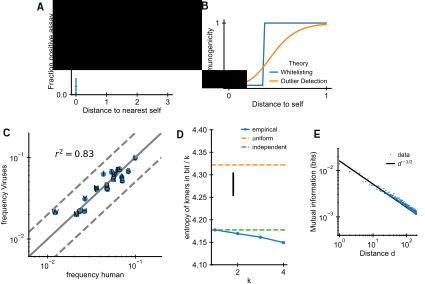
\includegraphics{figure1}
     \caption{
         {\bf Testing prior models of self/non-self peptide discrimination}
         (A, B) Typical models for determining which non-self peptides the immune systems targets, a depletion zone model where peptides close to self are whitelisted and other peptides are detected with uniform probability and an outlier detection model where more alien peptides are prioritized.
         (C) Response likelihood to foreign epitopes as a function of their distance to the nearest self peptide. Data: All 9mers from IEDB using ELISPOT assay.
         (D) A strong correlation is shown between the frequency of amino acid use in the human and viral proteome.
         (E) Entropy in bits as a function of $k$-mer length for a uniform, independent site model and empirical data.
         (F) Pairwise mutual information between amino acids at different distances. 
     \label{figure1}
     }
\end{figure*}


\subsection{Immune discrimination -- probabilistic classification or whitelisting?}

 To reason about how the logic of immune discrimination might impact the degree to which epitope immunogenicity depends on distance to self, it is insightful to draw an analogy to the theory of classification algorithms. Probabilistic classification between two sets of sequences can be achieved based on differences in sequence features. This is the common setting in machine learning: given a training set with items of each class learn a general classifier using statistical features that allow discrimination. Alternatively, when the sequences cover the space of all possible sequences sparsely, such that overlap between the two sets is rare, discrimination can also be achieved by whitelisting all sequences of one of the sets. The latter is memorization instead of generalization.

Whitelisting is the canonical logic that has been ascribed to immune discrimination and is supported mechanistically by central and peripheral tolerance. The hypothesis that immune discrimination also involves probabilistic classification has also been put forward \cite{Wortel2020}. Foreign peptides and self-peptides come from different proteomes, so there is some plausibility to the hypothesis that they might differ in sequence statistics and the immune system might consequently have evolved to exploit them. A probabilistic classification view of immune discrimination, is moreover compatible with the empirical usefulness of aligning neoantigens to pathogen epitopes to predict immunogenicity \cite{Luksza2017,Richman2019}.

In both scenarios we expect immunogenicity to increase with distance to self. Probabilistic classification acts as a mechanism to detect foreign peptides as ‘outliers’ relative to the distribution of self-peptides. Therefore, we would expect immunogenicity to increase continuously as we move farther away from self (Fig.~\ref{figure1}A). For a whitelisting strategy we expect no reactivity to antigens below a threshold level of similarity (Fig.~\ref{figure1}B), which value depends on the discriminatory power of the immune system between similar antigens given receptor cross-reactivity.

In the context of cancer, the immune system, at least sometimes, recognizes antigens that differ by a single mutation. Is this the exception that confirms the rule? To answer this question, we sought to understand how the immunogenicity of pathogen-associated antigens depends on their distance to self. We analyzed data from the Immune Epitope Database (IEDB), a curated database of antigens \cite{Vita2019}. The database contains data from a range of different T cell recognition assays. We found that different assays differed greatly in the fraction of overall reported positives, and in the proportion of positive assays for foreign peptides with exact matches in the self-proteome (Figure S1). Given incomplete clonal deletion we expected assays such as peptide-MHC (pMHC) binding that assess specific binding instead of a more functional readout to have high positivity rates even for epitopes found in self, and our results supported this expectation. We consequently focus our further analysis on a single assay (ELISPOT), which showed the smallest odds ratio between positive assays overall and peptides with exact matches (Figure S1). The sensitivity of this assay to peripheral tolerance is supported by an experimental study showing differences in response frequencies following depletion of regulatory T cells \cite{Bonertz2009}. We next aligned all foreign epitopes to their nearest self-peptide by edit distance, using an exact and fast hashing-based algorithmic approach (Material and Methods). We then calculated the fraction of epitopes at different distances to self that are immunogenic (Fig.~\ref{figure1}C). While epitopes identical to peptides found in the human proteome are less immunogenic, as expected, remarkably there are many epitopes that differ from self by a single amino acid which are immunogenic. Moreover, in contrast to theoretical expectations, we found that the most dissimilar peptides (distance 3+) are recognized with a lower frequency than peptides at distance of 1 or 2 amino acids away from self. Our analysis thus suggests the immune system preferentially focuses on regions of the antigen landscape close to self, even though farther, more dissimilar from self-peptides may be available to be recognized.

This surprising finding prompted us to ask quantitatively how the biophysics of protein statistics might have shaped the evolution of adaptive immune recognition. As a starting point, we compared amino acid usage between host and pathogen proteomes. We compared the amino acid usage using reference proteome data on the human proteome and the proteome of all human viruses. To create a non-redundant set of peptides, we pre-clustered the dataset using MMSeqs2 which reduces oversampling of specific viruses or protein families (Material and Methods). We found that amino acid usage is largely similar between the human and viral proteomes (Fig.~\ref{figure1}C). Is there higher order statistical structure in peptide space that might increase discriminability? For short $k$-mers we can directly determine the entropy of the distribution of $k$-mers from empirical counts. Applying a state-of-the art entropy estimation algorithm to the data reveals the presence of additional statistical structure beyond the constraints on amino acid usage, as seen by a consistent decrease in entropy rates for larger $k$ (Fig.~\ref{figure1}D). For $k>5$ the direct entropy estimation becomes challenging due to increased under sampling, and we instead analyze pairwise mutual information of amino acids at different distances (Fig.~\ref{figure1}E). We find that while the mutual information even for neighboring amino acids only reaches a modest maximal value of ~0.13 bit, correlations in amino acid usage are long-ranged, with mutual information decaying with distance roughly as a power-law of slope -0.5.

 \begin{figure*}
    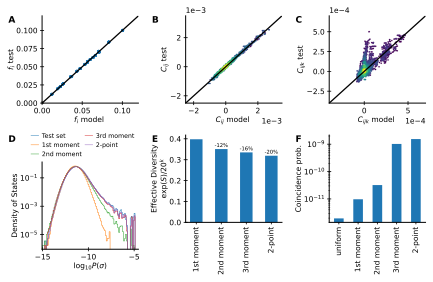
\includegraphics{figure2}
        \caption{{\bf Maximum entropy model predicts peptide statistics.}
        A maximum entropy model with third order compositional constraints and second order pairwise constraints on amino acid covariations captures the statistics of the human proteome. (A-C) Comparison of connected correlation functions in the test set with model predictions. (D,E) Density of states relative to the full energy function of models with different types of constraints. (F) Reduction in effective diversity of the peptide distribution resulting from imposing different constraints. The cumulative percentage reduction of effective diversity relative to the first moment model is indicated for each of the nested models. (G) Probability of coincidences in the different models, .
    \label{figure2}
    }
 \end{figure*}

\subsection{A statistical physics framework for probabilistic antigen classification} 

Prompted by these findings, we set out to use a maximum entropy framework as a principled way to include increasingly detailed statistical structure into a series of nested generative models of peptide statistics. This approach constrains certain statistical observables to equal their empirical values, while otherwise keeping the probability distribution as random as possible. We fit the parameters to the data using Boltzmann machine learning \cite{Ackley1985}. In short, we iteratively estimate empirical means of observables using Monte Carlo sampling for the current model parameters and then update model parameters to minimize the discrepancy between these estimates and their empirical counterparts (Materials and Methods).

We have constructed a hierarchy of such models to assess the significance of different constraints. We have found that a satisfactory model of 9mers drawn from the human proteome is provided by fitting the moments of the amino acid composition of peptides up to third-order, together with distance-dependent 2-point couplings. Taken together, these constraints produce a model that recapitulates key statistical features of the data (Fig.~\ref{figure2}A-C). By construction, the fitted model reproduces the average frequencies $f_i(\alpha)$ of finding amino acid $\alpha$ at position $i$ (Fig.~\ref{figure2}A), as well as the connected two-point correlation function (Methods) (Fig.~\ref{figure2}B). As a test of the model, we compare predicted and empirical connected three-point correlation functions (Fig.~\ref{figure2}C) and find good agreement. Moreover, the density of states is self-consistent between model and data (Fig.~\ref{figure2}D,E).

To quantify how different constraints reduce the diversity of the ensemble of peptides, we calculate the entropies  of the modelled distributions using thermodynamic integration (Material and Methods). Defining diversity as an effective number of equally likely peptides (i.e. as the exponential of the entropy), we find that global amino acid usage biases reduce diversity by 60\%, while further constraints collectively reduce diversity by an additional 20\% (Fig.~\ref{figure2}F). While this reduction in diversity as measured by entropy is relatively modest, the inclusion of higher-order constraints is important for other measures. For example, we find the probability with which two randomly drawn peptides coincide increases by orders of magnitude when including the additional constraints (Fig.~\ref{figure2}F). Note that the probability of a coincidence is equal to $\sum_{\B \sigma} P(\B \sigma)^2$, and thus puts larger weight than the entropy on the upper tail of probabilities. The increase of coincidences is thus linked to a heavy tail of highly likely sequences in the higher-order models (Fig.~\ref{figure2}D,E).


\begin{figure*}
    \begin{center}
        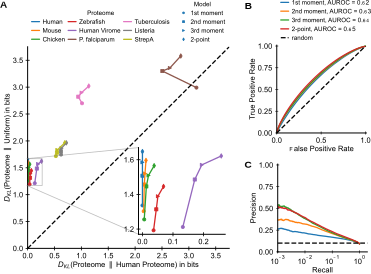
\includegraphics{figure3}
    \end{center}
    \caption{
        {\bf Divergence between peptides from different proteomes.}
        (A) Kullback-Leibler divergences between peptide distributions of different pathogen proteomes relative to human host peptides and relative to a uniform distribution over all peptides. For each proteome we show the statistical distance calculated according to a nested set of models including a different number of constraints. The inset shows a zoom on the set of proteomes close to the human statistics. (B, C) Performance of the models as classifiers. (B) Sensitivity-specificity tradeoff curve for various models. (C) Precision-recall characteristics at a 10-fold excess of self-peptides.
    \label{figure3}
    }
\end{figure*}

\subsection{Most peptide distributions biases are shared between hosts and pathogens}

We next compared proteome statistics from model organisms across different branches of jawed vertebrates: human and mouse as two examples of animals, chicken as an example of a bird, and zebrafish as an example of a jawed fish. We also compared them against a set of pathogen proteomes: a collection of human viruses (individual viral proteomes are too small for reliable statistical analyses), several pathogenic bacterial species, as well as a parasite (Plasmodium falciparum causing Malaria). For each proteome, we fit the same series of maximum entropy models to capture their statistical structure in increasing detail. We then use thermodynamic integration to quantify the statistical distinguishability of each proteome relative to the human proteome in terms of a Kullback-Leibler divergence. The Kullback-Leibler divergence is equal to the expected log-likelihood ratio for drawing a peptide from the pathogen distribution versus the human distribution. 

We find that with a few notable exceptions statistical divergence is small (Fig.~\ref{figure3}A). We also calculate the divergences with respect to a uniform distribution. We find that natural peptides are substantially easier to differentiate from completely random -mers than from natural peptides from a different proteome. This shows that a large fraction of biases in primary sequence statistics are shared among proteomes. Comparing the divergences across the model hierarchy we find that constraints beyond amino acid usage only modestly increase statistical distances. In most cases the inclusion of additional constraints increases the distance from random peptides more than from human peptides, implying a large degree of conservation of these constraints across proteomes. Bacterial proteomes differ more substantially, but their divergence is still smaller than 1 nat in all cases. The largest divergence is found for the parasite Plasmodium falciparum, which might be a result of the known AT bias of its genome \cite{Hamilton2017}.

Given the small Kullback-Leibler divergence we expect limited performance of these models as classifiers. Indeed, we find modest classification performance as assessed by the area under the receiver operating curve (Fig.~\ref{figure3}B). However, similarly to how the small reduction in entropy went along with a large increase in coincidence probability, discriminability in the tails is more substantial as highlighted in a precision-recall plot (Fig.~\ref{figure3}C). For example, among the top 1\% of most distinguishable viral peptides, precision is roughly four-fold above chance using the higher order models, when host peptides are in 10-fold excess. Viral proteome sizes are in the $10^3$-$10^4$ amino acid range (higher for DNA then RNA viruses). Assuming 10\% of peptides can be presented, the top 1\% corresponds to the top few peptides.



\begin{figure*}
    \begin{center}
        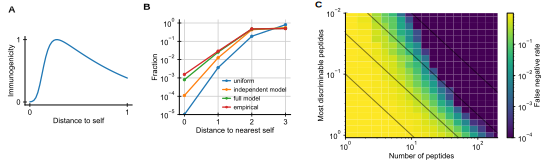
\includegraphics{figure4}
    \end{center}
    \caption{
        {\bf A theory of immune discrimination in the light of shared proteome biases.}
        (A) Distribution of distances to the nearest self peptide for peptides from human viruses, their modelled distribution, and a null model with a uniform distribution over all $20^9$ kmers. (B) Odds ratio with which viral peptides at a certain distance to self are encountered. (C) Schematic of a shell-model of non-self peptide recognition where the immune systems biases its search based on more likely “close to self” peptides. 
    \label{figure4}
    }
\end{figure*}

\subsection{Viral peptides are close to self suggesting a shell model of immunogenicity}

An important consequence of the shared sequence biases between self and non-self is to make (near-)coincidences, and therefore matches by the immune system, between peptides much more likely. To quantify this effect, we calculate the distance to the nearest self-peptide for a collection of immune epitopes from IEDB (for 9mers). While the reduction in peptide diversity is on the order of tens of a percent, we find the probability of precise coincidences is increased by more than two orders of magnitude compared to the expectation under a uniform model, and near-coincidences differing by a single amino acid are also heavily enriched (Fig.~\ref{figure4}A).

This provides a possible rationale for a "shell model" of immunogenicity (Fig.~\ref{figure4}B), where the immune system preferentially targets epitopes of intermediate distance to self. A consequence of this model is a new interpretation of the role of positive and negative selection in thymic selection. Instead of a system where the role of negative selection is strict whitelisting and positive selection solely serves to eliminate T cells that do not recognize any host HLA molecules, our theory suggests that thymic selection trains T cells to recognize likely peptides that are close to self, while eliminating only a small subset of peptides that are broadly expressed in somatic tissue.

We can also use our model to quantify under which conditions a quorum sensing strategy can work, i.e. a decision-making strategy relying not on the presence of a single peptide, but  different peptides, simultaneously present on a cell or in a tissue site. While in practice there will be constraints on how reliably different cells can pool information to coordinate their decision, here we put a theoretical upper bound on the performance of quorum sensing. To this end, we calculate the distribution of cumulative likelihood ratios for  randomly sampled peptides from either the pathogen or host proteome. We then determine the achievable false negative rate by a decision rule at a fixed false positive rate. We find that more than a hundred peptides are needed for reliable discrimination (Fig.~\ref{figure4}B). However, most of the statistical power stems from a much smaller subset of peptides: if, for example, only the top 1\% of peptides with the largest likelihood ratios are considered the number of peptides needed for reliable responses drops substantially to ~10. This order of magnitude is consistent with the observed immunodominance of a small set of peptides \cite{REF NEEDED}, implying immunodominance may be explained by quorum sensing of peptides at the tail of a pathogens distribution of peptide statistics.

\section{Discussion}

While we typically think of self and non-self peptide discrimination as either a whitelisting of self-peptides within a uniform distribution of possible antigens or learning the rules to statistically distinguish self and non-self peptide distributions, we show that self and non-self peptides are generated from similar peptide distribution. However, when comparing pathogen and host derived peptides, we find no clear statistical differences. The implication is that an efficient immune system would, in the optimal case, leverage this similarity to focus on peptides that are close to self rather than those that are far from self. Indeed, we find empirical support for this prediction in the limited immunogenicity data available to date, supporting the notion that the immune systems preferentially target viral epitopes close to self, rather than those that are the most foreign or alien. Moreover, a consequence of these shared biases is that only a small number of antigens are needed for efficient pathogen recognition, offering a novel theoretical explanation for immunodominance.

If further corroborated, this shell model might be of relevance for both vaccine selection and cancer immunotherapy. Mutation derived neoantigens that are only one mutation away from self might not be that special in the landscape of epitopes the immune system encounters and designing a vaccine to prioritize peptides farthest from self might not offer the obvious advantage one might expect. Due to underlying shared biases many more antigens from pathogens are closer to self than naively expected. Evolutionarily this would make sense. Why would natural selection anticipate the need to prioritize far-from-self viral peptides when it rarely encounters them. Hopefully our approach will stimulate a reassessment of what approaches evolution might have selected to discriminate self from non-self and why, while also providing testable prediction that can be used in novel immunotherapies and emerging antiviral strategies.

\section{Material and Methods}

\subsection{Model construction and fitting}
We propose to use a maximum entropy framework as a principled way to include increasingly detailed statistical structure into a series nested models of peptide statistics. Using this approach we constrain a set of statistical observables $\langle f_\mu(\boldsymbol \sigma)\rangle$ to equal their empirical values $\bar{f_\mu}$, while otherwise keeping the probability distribution as random as possible. Mathematically, this means choosing the probability distribution to maximize the Shannon entropy
\begin{equation}
    S[P(\B \sigma)] = - \sum_{\B \sigma} P(\B \sigma) \log P(\B \sigma),
\end{equation}
subject to the normalization constraint $\sum_{\B \sigma} P(\B \sigma) = 1$, and constraints that enforce the equality of modelled and empirical observables
\begin{equation}
    \langle f_\mu(\boldsymbol \sigma)\rangle = \sum_{\boldsymbol \sigma} P(\boldsymbol \sigma) f_\mu(\boldsymbol \sigma) = \bar{f_\mu}.
\end{equation}
Optimizing with respect to the normalization constraint yields a Boltzmann distribution of the form,
\begin{equation}
    P(\boldsymbol \sigma) = \frac{1}{Z} \exp\left[ -E(\B \sigma) \right],
\end{equation}
where
\begin{equation}
 E(\B \sigma) = \sum_{\mu=1}^K \lambda_\mu f_\mu(\boldsymbol \sigma),
\end{equation}
is a sum of terms involving each constraint, which is called the energy in statistical mechanics, and 
\begin{equation}
    Z = \sum_{\B \sigma} \exp \left[ - E(\B \sigma) \right]
\end{equation}
is a normalization factor, called the partition function.

We fit the parameters $\lambda_\mu$ to the data using Boltzmann machine learning \cite{Ackley1985}. In short, we iteratively estimate $\langle f_\mu(\B \sigma)\rangle$ using Monte Carlo sampling for a given set of model parameters and then update parameters to minimize the discrepancy between estimated and empirical observables.

A common choice is to constrain the one and two-point frequencies
\begin{align}
    f_i^\alpha(\B \sigma) &= \sigma_i^\alpha, \\
    f_{ij}^{\alpha\beta}(\B \sigma) &= \sigma_i^\alpha \sigma_j^\beta,
\end{align}
where $\sigma_i^\alpha = 1$ if the amino acid at site i is of type $\alpha$ and zero otherwise.
This leads to a maximum entropy probability distribution that takes the form of a disordered Potts model,
\begin{equation}
    E(\boldsymbol \sigma) = - \sum_{i=1}^L \sum_{\alpha = 1}^{20} h_i^\alpha \sigma_i^\alpha - \sum_{i<j}^L \sum_{\alpha,\beta = 1}^{20} J_{ij}^{\alpha \beta}  \sigma_i^\alpha \sigma_j^\beta.
\end{equation}

Given that many biases are compositional in nature we can also consider a simpler model that only involves a global constraint on the covariation of the total count of amino acids of different types:
\begin{align}
    n^\alpha(\B \sigma) &= \sum_i \sigma_i^\alpha, \\
    n^{\alpha\beta}(\B \sigma) &= n^\alpha(\B \sigma) n^\beta(\B\sigma) = \left(\sum_{i=1}^L \sigma_i^\alpha\right) \left(\sum_{j=1}^L \sigma_j^\beta\right).
\end{align}
This leads to a maximum entropy probability distribution that takes the form
\begin{equation}
    E(\boldsymbol \sigma) = - \sum_{\alpha=1}^{20} h^\alpha n^\alpha -  \sum_{\alpha,\beta = 1}^{20} J^{\alpha \beta} n^\alpha n^\beta,
\end{equation}
i.e. a model that only involves global couplings between amino acids independent of their distance.


The parameters are updated by iterative scaling,
\begin{equation}
    \lambda_\mu^{t+1} = \lambda_\mu^t + \epsilon_\mu^t \log \left( \frac{\langle f_\mu \rangle}{\bar{f_\mu}} \right),
\end{equation}
where $\epsilon_\mu^t$ represents a learning rate (which generally can be coordinate dependent and time-varying).
%The parameters are updated by gradient ascent,
%\begin{equation}
%    \lambda_\mu^{t+1} = \lambda_\mu^t + \epsilon_\mu^t \left(\langle f_\mu \rangle  - \bar{f_\mu}\right),
%\end{equation}
%where $\epsilon_\mu^t$ represents a learning rate (which generally can be coordinate dependent and time-varying).

\subsection{Calculation of entropy by thermodynamic integration}
Once we have fitted the model parameters we can calculate the entropy of the distribution $P(\B \sigma)$. To do so we use the identity
\begin{align}
    S &= - \sum_{\B \sigma}  P(\B \sigma) \log P(\B \sigma),  \\
      &= \langle E(\B \sigma) \rangle - F, \quad F = - \log Z.
\end{align}
The mean energy can be calculated directly from Monte Carlo samples. To calculate the free energy we use thermodynamic integration as follows \cite{Marchi2019b}: We express the energy with respect to a reference energy $E_{ref}(\B \sigma)$ as $E(\B \sigma) = E_{ref}(\B \sigma) + \Delta E(\B\sigma)$, where the reference energy is choosen such that $F_{ref}$ can be calculated analytically. We define the perturbed energy function
\begin{equation}
    E_\alpha(\B \sigma) = E_{ref}(\B \sigma) + \alpha \Delta E(\B\sigma),
\end{equation}
which scales the contribution of the energy beyond the reference model.
To obtain the free energy we use the identity
\begin{equation}
    F(1) = F_{ref} + \int_0^1 \ud \alpha F'(\alpha).
\end{equation}
Note that
\begin{equation}
    F'(\alpha) = - \langle \Delta E(\B \sigma) \rangle_{\alpha},
\end{equation}
which allows us to approximate the integrand by Monte Carlo simulations. We numerically evaluate $F'(\alpha)$ for evenly spaced $\alpha \in [0, 1]$ and calculate the integral by Simpson's rule. Calculating the entropy in this way allows us to determine the reduction in the effective diversity in sequences implied by including different constraints. 

\clearpage

\begin{figure}
     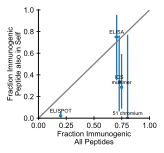
\includegraphics{figureS1}
     \caption{
         {\bf Differences between assays measuring immunogenicity.}
         For each assay the fraction of peptides with positive T cell recognition assay among foreign peptides found identically in the human reference proteome is plotted against the same fraction in all foreign peptides (Data from IEDB). Some assays such as multimer binding are nearly always positive when found in the database regardless of any potential tolerance against peptides also found in self. These assays are thus less useful for assessing functional immunogenicity of peptides.
     \label{figureS1}
     }
\end{figure}

\begin{figure}
     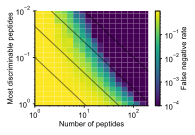
\includegraphics{figureS2}
     \caption{
         {\bf Empirical constraints on discrimination by quorum sensing across peptides.}
        How many peptides allow reliable quorum sensing? Achievable false negative rates as a function of the number of peptides at a fixed false positive rate equal to $10^{-3}$. Most of the discrimination ability is driven by a smaller subset of most discriminable peptides. The black lines show a  scaling for reference.
     \label{figureS2}
     }
\end{figure}




\bibliographystyle{apsrev}
\bibliography{library}


\end{document}
